%%%%%%%%%%%%%%%%%%%%%%%%%%%%%%%%%%%%%%%%
% introduction

Active perception enables a robot to reason on how to efficiently acquire more (task-related) information in a noisy environment in order to complete a task at hand.
The task we pursue in this work is to enable a robot to reason on how to autonomously combine visual and haptic information to identify the shape of household objects that can be successively grasped and manipulated by a human-sized hand. 

Our approach is to formalise the problem of shape representation as a problem of linear regression, in which a Gaussian Process (GP) is employed to learn a probabilistic model of the object. The GP allows us to build a \emph{maximum a posteriori} (MAP) estimation of the object's surface described as an implicit function, $f(\mathbf{x})=0$, (the 0-levelset of the approximating function) as well as to constrain the learnt function on visual and haptic clues in order to converge to the real shape of the object. To enable the robot to select best-next (exploration) actions, we construe the function $f(\mathbf{x})$ as a manifold and we grow an exploration tree, similar to the AtlasRRT described in~\cite{Jaillet2013Path}, which is biased to visit uncertain region of the object's surface.

This section proceeds as follows. We firstly introduce the general formulation for GPR for implicit surfaces. We then show how to compute first-order quantities from the GP (surface normals) which are essential to locally parametrise a manifold (Atlas). Finally, we present how to build a sample-based exploration on the manifold to visit regions of the object's surface that are more promising to reduce the global model uncertainty.


\todo[]{Equipment specification and assumptions have been removed. They should be move later when describing the experimental setup.}
%%%%%%%%%%%%%%%%%%%%%%%%%%%%%%%%%%%%%%%%%
%\subsection{Equipment specification}
%\label{sec:equipment}
%\todo[inline]{Equipment list and specifics missing}
%The vision  system should  be able  to provide  an initial  guess on  the object
%location  and  observation  points  on  the  surface.  This  is  not  an  strict
%requirement, since  one might  be completely blind  and still  recognize objects
%around \citep[e.g.]{Petrovskaya2011Global}.  However, the use of  an initial set
%of observation can  be done quickly using  RGBD sensors to speed  up the overall
%process.
%
%It is true that mounting the camera as the end-effector of a robot might allow a
%full object scanning, but there might be  cases where this might not be possible
%either  due to  reaching limitations  or  even sensing  capabilities on  reduced
%spaces.
%
%%%%%%%%%%%%%%%%%%%%%%%%%%%%%%%%%%%%%%%%%
%\subsection{Assumptions}
%\label{sec:limitations}
%\todo[inline]{Needs rewording, expansion}
%
%We assume that a point cloud of a segmented object is provided. However, we provide an optional pre-processing step that shows a reasonably way to do it when the object model is unkown.
%
%Workspace. This is not to be thought as the workspace of a robot, but of the strategy algorithm that works on top of the object shape model. That is, we assume that we are modelling and exploring household objects that can be grasped and manipulated using a human-sized hand. This is specially useful in cases where the predicted shape is not bounded using the given observations, so this workspace will shrink the predicted shape to prevent the robot from going to an empty space, or worst, hitting undesirebly. 
%
%We consider contact to appear when the force torque sensor measures a value higher than $1$N. The robot motion is set slow such that inertial forces are not reflected on the measurements. This is done for safety reasons, since in the phase when the robot is approaching, there is a stop signal if this threshold is superated.
%
%%%%%%%%%%%%%%%%%%%%%%%%%%%%%%%%%%%%%%%%%
%\subsection{Problem statement}
%\label{sec:problem}
%\todo[inline]{Needs more elaborate explanations}
%
%Considering the equipment limitations~\ref{sec:equipment} and the assumptions~\ref{sec:limitations}, the problem for which we propose a solution can be stated as:
%
%Given a point cloud of an object, $\mathcal{O}$, find a suitable represention for the shape that can be exploited for tasks such as object identification and grasping, and a coherent strategy to improve the representation independent of external references, i.e. intrinsic or exploiting the representation, and flexible enough to generate different exploratory actions such as poking points and sliding paths.
%
%Many robotics applications suffer of the lack of complexity in the model used to represent the problem at hand. A new trend in robotics is to encode states and observations in a probabilistic framework to cope with novelty in the face of uncertainty. Our work follows such an approach in the sense that we integrate, in an online fashion, multi-sensory inputs (here vision and tactile clues) in a stochastic model.
%
%This section formulates the problem of shape modelling of unknown objects (starting from a visual clue) while simultaneously planning information-gathering actions to complete our knowledge of the object to manipulate. By unknown objects, we mean that the robot does not have priory knowledge of the geometrical features of the object to be explored.  

%%%%%%%%%%%%%%%%%%%%%%%%%%%%%%%%%%%%%%%%
\subsection{Gaussian Process Regression for Implicit Surfaces}
\label{sec:gpr}
%A Gaussian Process (GP) is a (finite) collection of random variables with a joint Gaussian distribution. 

\todo[]{There's some notation conflict to fix, on later sections S is the implicit object surface.}
Let $\mathcal{S}$ be a training dataset of $N$ observations, $\mathcal{S}=\{(\mathbf{x}_i, y_i)|i=1,\dots,N\}$, where $\mathbf{x}_i\in\mathbb{R}^n$ denotes the $i^{th}$ input vectors and $y_i\in\mathbb{R}$ the associated scalar output or target.  We collect the $N$ inputs vectors in a $n\text{ x }N$ matrix $X$ and the output target in a $N\text{ x }1$ vector $\mathbf{y}$, so that we can rewrite the training dataset in a more compact way as $\mathcal{S}=(X,\mathbf{y})$. We are interested in making inference about the mapping function $f:\mathbb{R}^n\rightarrow\mathbb{R}$ between the input vectors and the targets. We assume a linear regression model
$$
y_i=f(\mathbf{x}_i)+\epsilon
$$
where $\epsilon\thicksim\mathcal{N}(0,\sigma_n^2)$ is an independent identically distributed Gaussian noise with zero-mean and variance $\sigma_n^2$. 

A Gaussian Process framework for regression (GPR) is a common choice to approximate $f(\mathbf{x})$, in which the targets $y_i$ are assumed to be drawn from a zero-mean multi-variate Gaussian distribution with a covariance matrix which is a function of the input vectors. Therefore the output distribution can be written as
\begin{eqnarray}
\label{eq:gpr}
(y_1,\dots,y_N|\mathbf{x}_1,\dots,\mathbf{x}_N)\thicksim\mathcal{N}(0,K(X,X)+\sigma_n^2I)
\end{eqnarray}
The covariance function expresses somehow the notion of nearness or similarity, for which points in the input space $\mathbb{R}^n$ that are close would likely produce similar outputs. The choice of a kernel is a crucial ingredient for a GP and a vast part of the literature has investigated this problem, sometimes referred as the \emph{kernel trick}. Following previous works on implicit surface estimations we chose the \emph{thin plate} kernel, which is defined as
\begin{eqnarray}
\label{eq:thinplate}
K(\mathbf{x}_i,\mathbf{x}_j)=2\|\mathbf{x}_i-\mathbf{x}_j\|_2^3-3R\|\mathbf{x}_i-\mathbf{x}_j\|_2^2+R^3
\end{eqnarray}
where $\|\mathbf{a}\|_2=\sqrt{\mathbf{a}^\top\mathbf{a}}$ and $R=\max(\|\mathbf{x}_i-\mathbf{x}_j\|_2),\forall\mathbf{x}_i,\mathbf{x}_j\in\mathcal{S}$, is the largest pairwise distance between the input vectors in the training dataset $\mathcal{S}$. To improve the prediction performance of the GP with a thin plate kernel is useful to divide the training dataset in three disjointed subsets, namely $\mathcal{S}^0=\{(\mathbf{x}_i,y_i)\in\mathcal{S}|y_i=0\}$ are the inputs labelled as ``on the object's surface'', $\mathcal{S}^+=\{(\mathbf{x}_i,y_i)\in\mathcal{S}|y_i=+1\}$ and $\mathcal{S}^0=\{(\mathbf{x}_i,y_i)\in\mathcal{S}|y_i=-1\}$ are artificial inputs, respectively, laying outside and inside the object's surface. We then can rewrite the training dataset as $\mathcal{S}=\mathcal{S}^0\cup\mathcal{S}^+\cup\mathcal{S}^-$ and its cardinality $N=N^0+N^++N^-$ as the sum of the respective cardinalities.

Given a new point $\mathbf{x}_*$, it is possible to query the GP to compute the estimate of $y_*=\bar{f}(\mathbf{x}_*)$ with a measure of confidence expressed by its associated variance $\mathbb{V}[y_*]$ by deriving the following equations from Eq.~\ref{eq:gpr}:

\begin{eqnarray}
\label{eq:gpr_mu}
y_*=\mathbf{k}_*^\top(K+\sigma_n^2I)^{-1}\mathbf{y}
\end{eqnarray}

\begin{eqnarray}
\label{eq:gpr_var}
\mathbb{V}[y_*]=k(\mathbf{x}_*,\mathbf{x}_*)-\mathbf{k}_*^\top(K+\sigma_n^2I)^{-1}\mathbf{k}_*
\end{eqnarray}
Notice that we have introduced a more compact notation where, for a single query point $\mathbf{x}_*\in\mathbb{R}^n$, $\mathbf{k}_*=K(\mathbf{x}_*,X)$ is the $N\text{ x }1$ covariance vector between the query point and the training dataset $X$. Similarly, $K=K(X,X)$ is the covariance matrix evaluated on the training dataset and $k(\mathbf{x}_*,\mathbf{x}_*)$ is a scalar value denoting the variance between the query point and itself.

\subsection{Gaussian process derivative}
\label{sec:gpr_der}

In the previous section we introduced a general formulation of GPR to describes implicit surfaces in terms of its mean (Eq.~\ref{eq:gpr_mu}) and variance (Eq.~\ref{eq:gpr_var}). We also shown that, given an query input $\mathbf{x}_*$ it is possible to predict its expected target value, $\bar{f}(\mathbf{x}_*)$ as well as its associated expected variance $\mathbb{V}[f(\mathbf{x}_*)]$. As described in~\cite{Rasmussen2006Gaussian}, a GPR can be utilised to make prediction on the gradient of the approximating function, $\mathbb{E}[f'(\mathbf{x})]$. In the case of implicit surface this information is equivalent to make an estimate of the normal surface at the evaluated point $\mathbf{x}_*$.\todo[]{add citation here}

The gradient estimation can be computed by using a mixed covariance function between function values and partial derivates. Given two input vectors $\mathbf{x}_i$ and $\mathbf{x}_j$ the mixed covariance function can be written as
$$
cov(f(\mathbf{x}_i), \frac{\partial f(\mathbf{x}_j)}{\partial\mathbf{x}})=\frac{\partial k(\mathbf{x}_i, \mathbf{x}_j)}{\partial\mathbf{x}_j}
$$
which is equivalent to calculate the vector of partial derivatives with respect to $\mathbf{x}_j$ of the original kernel function. The first partial derivate of the thin plate covariance can be written as
\begin{eqnarray}
\label{eq:gpr_der} 
\frac{\partial k(\mathbf{x}_i,\mathbf{x}_j)}{\partial\mathbf{x}_j}&=6(\mathbf{x}_i-\mathbf{x}_j)(\|\mathbf{x}_i-\mathbf{x}_j\|_2 + R)
\end{eqnarray}

For a single query point $\mathbf{x}_*$, we define 
$$
\frac{\partial K_*}{\partial\mathbf{x}}=\frac{\partial\mathbf{k}(X,\mathbf{x})}{\partial\mathbf{x}}\bigg|_{\mathbf{x}=\mathbf{x}_*}
$$ 
as the $N\text{ x }n$ mixed covariance matrix between the function values at the training points $X$ and the partial derivatives evaluated at the query point. 

Therefore, similarly to Eq.\ref{eq:gpr_mu}, the expected normal, $\mathbf{n}_*$, on the query input $\mathbf{x}_*$ can be computed by the following equation

\begin{eqnarray}
\label{eq:gpr_n}
\mathbf{n}_*=\mathbb{E}[f'(\mathbf{x})]=\frac{\partial K_*}{\partial\mathbf{x}}^\top(K+\sigma_n^2I)^{-1}\mathbf{y}
\end{eqnarray}
where $\mathbf{n}_*$ is a $n\text{ x }1$ vector.

\subsection{Local parametrisation of a manifold}\label{sec:atlas}

%Following the formulation in~\cite{Jaillet2013Path}, 

The GP for implicit function defined in Sec.~\ref{sec:gpr} defines a probabilistic representation of a unknown surface and therefore a global parametrisation of such a surface is not available. However we can interpret the surface as a manifold, $\mathcal{F}$, implicitly defined by a set of constraints such that $\mathcal{F}=\{\mathbf{x}\in\mathbb{R}^n|f(\mathbf{x})=0\}$. The manifold is represented as a collection of $k$-dimensional parameter spaces called charts.
Given a point $\mathbf{x}_i\in\mathbb{R}^n$ on the manifold, a chart $\mathcal{C}_i$ is defined as a local parametrisation of the orthogonal tangent space at $\mathbf{x}_i$. We denote $\mathbf{u}_p^i\in\mathcal{C}_i$ a parameter vector such that 
\begin{equation}
\label{eq:psi}
\mathbf{x}_p^i=\mathbf{x}_i+\Phi_i\mathbf{u}_p^i
%\mathbf{x}_j^i=\pmb{\phi}_i(\mathbf{u}_j^i)=\mathbf{x}_i+\Phi_i\mathbf{u}_j^i
\end{equation}
where $\Phi_i\in\mathbb{R}^{n\text{x}k}$ is an orthogonal basis for the tangent space to the manifold at $\mathbf{x}_i$ and $\mathbf{x}_p^i\in\mathbb{R}^n$ is a point laying on this tangent space reachable from $\mathbf{x}_i$ through the parameter $\mathbf{u}_p^i$. Notice that both points $\mathbf{x}_i$ and $\mathbf{x}_p^i$ are defined in $\mathbb{R}^n$; in the literature this $n$-dimensional space is sometime referred as the ambient space (here a 3D space) to distinguish it from the $k$-dimensional space of the manifold (2D), with $n > k > 0$.

To compute the tangent basis, $\Phi_i$, we make use of the estimated normal, $\mathbf{n}_i=\mathbb{E}[f'(\mathbf{x})]$, obtained by approximating the gradient of the GP at the point $\mathbf{x}_i$, as described in Sec.~\ref{sec:gpr_der}. Then we estimate $\Phi_i$ such that it satisfies the following linear system
$$
\left[
\begin{array}{c}
\mathbf{n}_i \\
\Phi_i^\top
\end{array}\right]\Phi_i
=
\left[
\begin{array}{c}
0 \\
I
\end{array}\right]
$$  
where $I$ identifies the $k\text{ x }k$ identity matrix.  

The chart $\mathcal{C}_i$ also defines a bijective map between parameters $\mathbf{u}_p^i\in\mathbb{R}^k$ and $n$-dimensional points on the manifold. The function $\psi_i(\mathbf{u}_p^i)=\mathbf{x}_p$ is known in the literature as the \emph{exponential map} and defines the relation between the parameter space of the chart $\mathcal{C}_i$ and any point on the manifold $\mathbf{x}_p$. Similarly, the \emph{logarithmic map} expresses the inverse relation, $\psi_i^{-1}(\mathbf{x}_p)= \mathbf{u}_p^i$.

A typical implementation of the exponential map makes use of Eq.~\ref{eq:psi} to move along the tangent space at $\mathbf{x}_i$ in the direction defined by the parameter vector $\mathbf{u}_p^i$, then it projects the point $\mathbf{x}_p^i$ on the object surface by solving the system of equations
\begin{align}
\label{eq:projection}
\begin{cases}
f(\mathbf{x}_p)&=0\\
\Phi_i^\top(\mathbf{x}_p-\mathbf{x}_p^i)&=0
\end{cases}
\end{align}
to find a point $\mathbf{x}_p$ that lays on the manifold and, therefore, on the estimated object surface. 

\subsection{Exploring a manifold}

In this work we aim to generate a path along an object surface, described as a manifold over a GP estimation, $\mathcal{F}$, that a robotic finger equipped with a F/T sensor can follow to gather new information about the shape of the object. Such an information will be then integrated in a probabilistic model (GP) in order to refine the manifold. The goal is to iteratively converge to a model of the object's shape in which the shape uncertainty becomes negligible. 

We build on the recent advances on sample-based techniques for asymptotically optimal exploration of a general manifold. Similarly to the work of~\cite{Jaillet2013Path} we use an RRT algorithm to construct a path on the manifold. However the major difference with their work is how we construct a chart around a given point $\mathbf{x}_i$ and how we select a new candidate node for the RRT algorithm.

Given a point $(\mathbf{x}_i, y_i\in\mathcal{S}^0$ such that $y_i=0$ we compute its estimated normal, $n_i$, using Eq.~\ref{eq:gpr_n} and the chart $\mathcal{C}_i$ as a disc centred in $\mathbf{x}_i$ with radius
$$
\rho=\frac{1}{\mathbb{V}[f(\mathbf{x}_i)]}
$$
which is inversely proportional to the expected variance of our model at point $\mathbf{x}_i$. This allows us to construct larger tangent space in region in which the confidence of the model is higher and thus to reduce the allowed exploring region when the model has less information. 

From the chart $\mathcal{C}_i$ we can randomly sample a finite set of $d$ candidate parameter vectors $\mathbf{u}_p^i$ with $p\in[1,\dots,d]$. Each parameter vector $\mathbf{u}_p^i$ encodes a direction of exploration from the central point $\mathbf{x}_i$ to a point $\mathbf{x}_p^i$ such that
$$
\|\mathbf{x}_i-\mathbf{x}_p^i\|_2=\rho
$$
laying on the circumference of the chart. Using the exponential map described in Sec.~\ref{sec:atlas}, we compute the projection $\mathbf{x}_p=\psi_i(\mathbf{u}_p^i))$ such that $\mathbb{E}[f(\mathbf{x}_p)]\approx0$ which leads us to points that are estimated to be on the object surface by our probabilistic model. An user-defined threshold $\epsilon$ can be set to modify the system of equations in Eq.~\ref{eq:projection} to
\begin{align}
\label{eq:approxprojection}
\begin{cases}
|f'(\mathbf{x}_p)|&\leq\epsilon \\
\Phi_i^\top(\mathbf{x}_p-\mathbf{x}_p^i)&=0
\end{cases}
\end{align}
where $f'(\mathbf{x}_p)=\mathbb{E}[f(\mathbf{x}_p)]$ and $|\cdot|$ is the absolute value function.

We then select the direction $\mathbf{u}_{p'}^i$ such that
$$
p'=\argmax_{p\in[1,\dots,d]}{\mathbb{V}[f(\psi_i(\mathbf{u}_p^i))]}
$$
to obtained a candidate target point $\mathbf{x}_{p'}$ ion the manifold. 

\begin{figure}[h]
    \centering
    \mbox
    {
        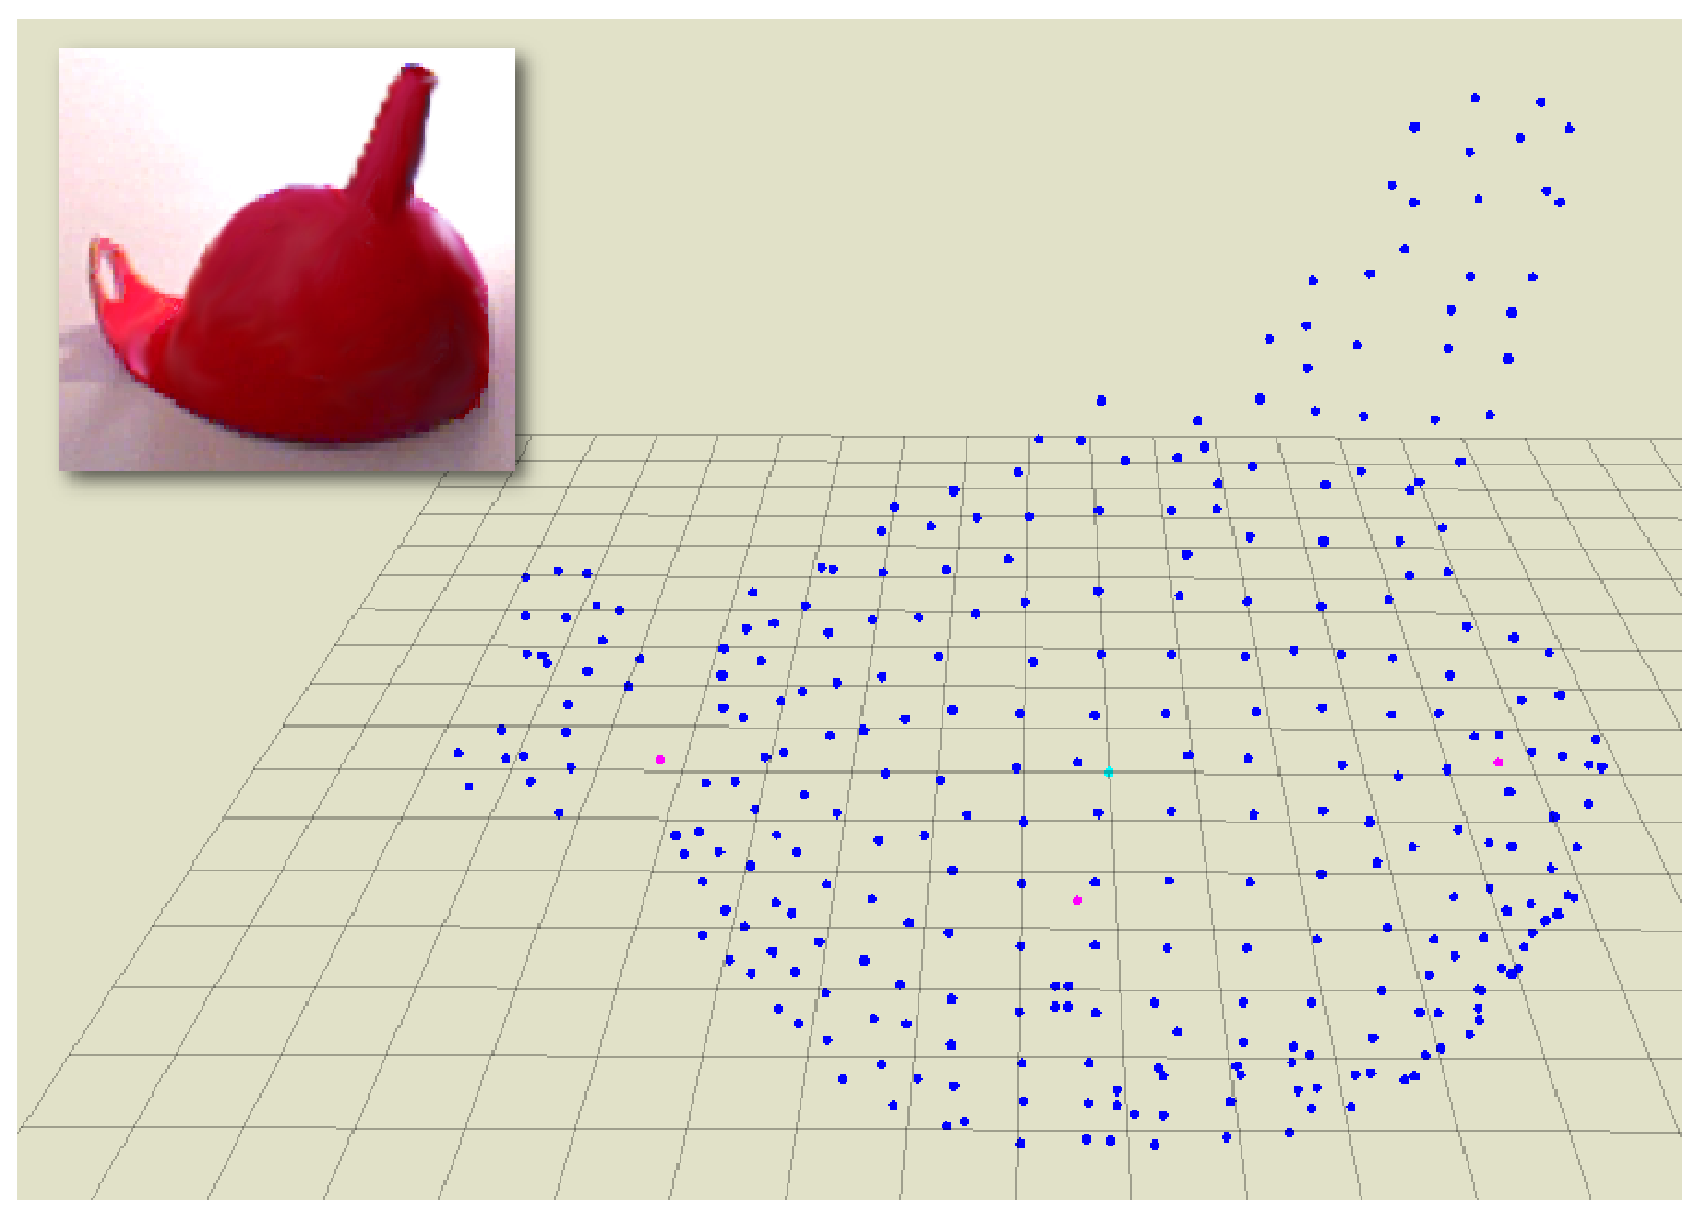
\includegraphics[width=0.45\linewidth]{funnelC.eps}
        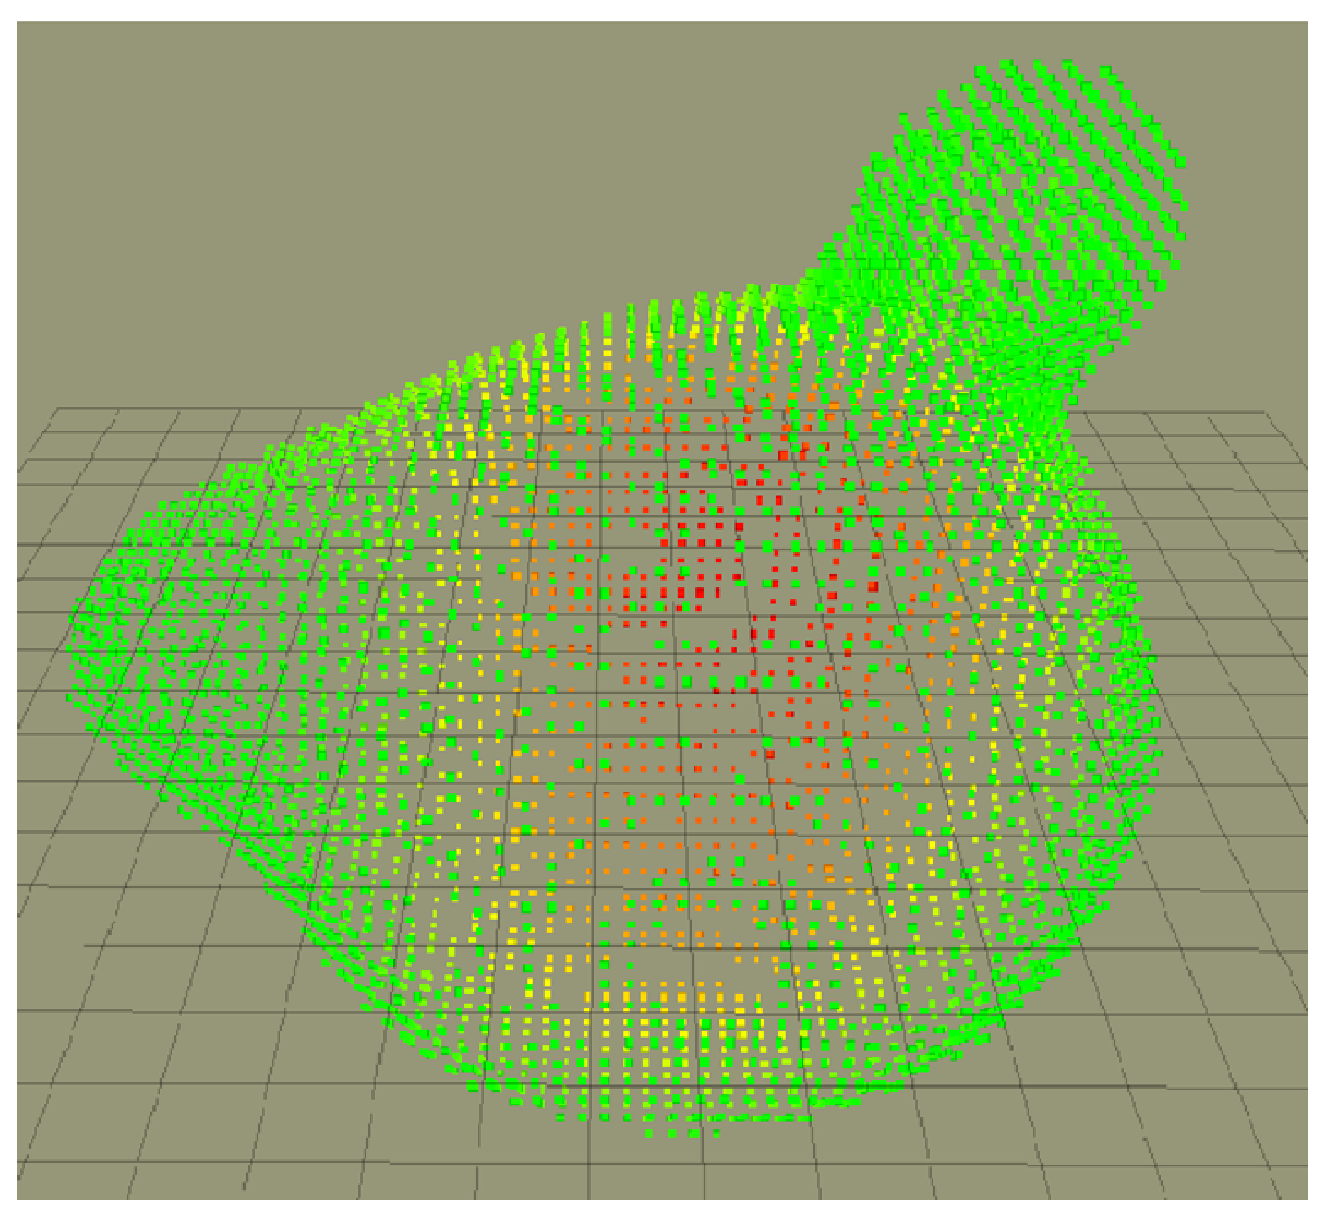
\includegraphics[width=0.45\linewidth]{funnelS.eps}
    }
    \caption{Gaussian Process regression on a funnel object. }
    \label{fig:GPfunnel}
    \todo[inline]{just added to see how it looks on the paper}
\end{figure}
\begin{figure}[h]
    \centering
    \mbox
    {
    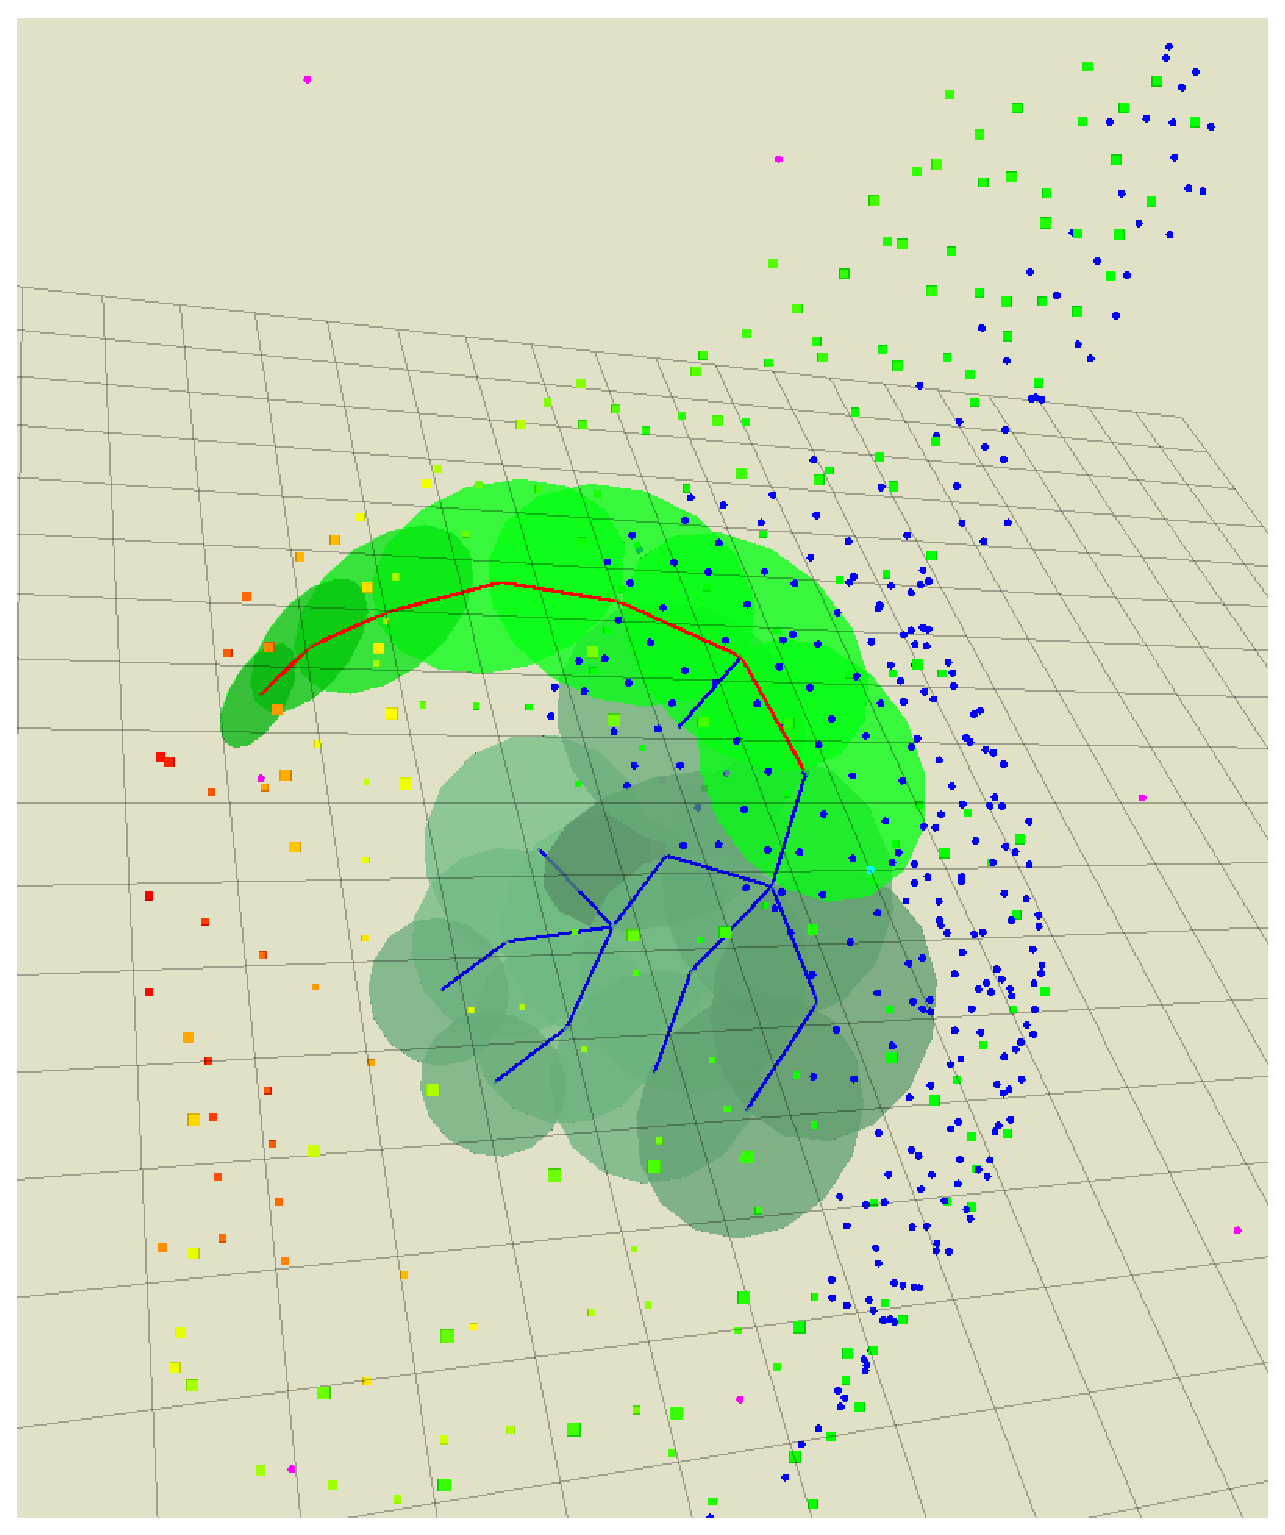
\includegraphics[width=0.45\linewidth]{funnelRRT.eps}
    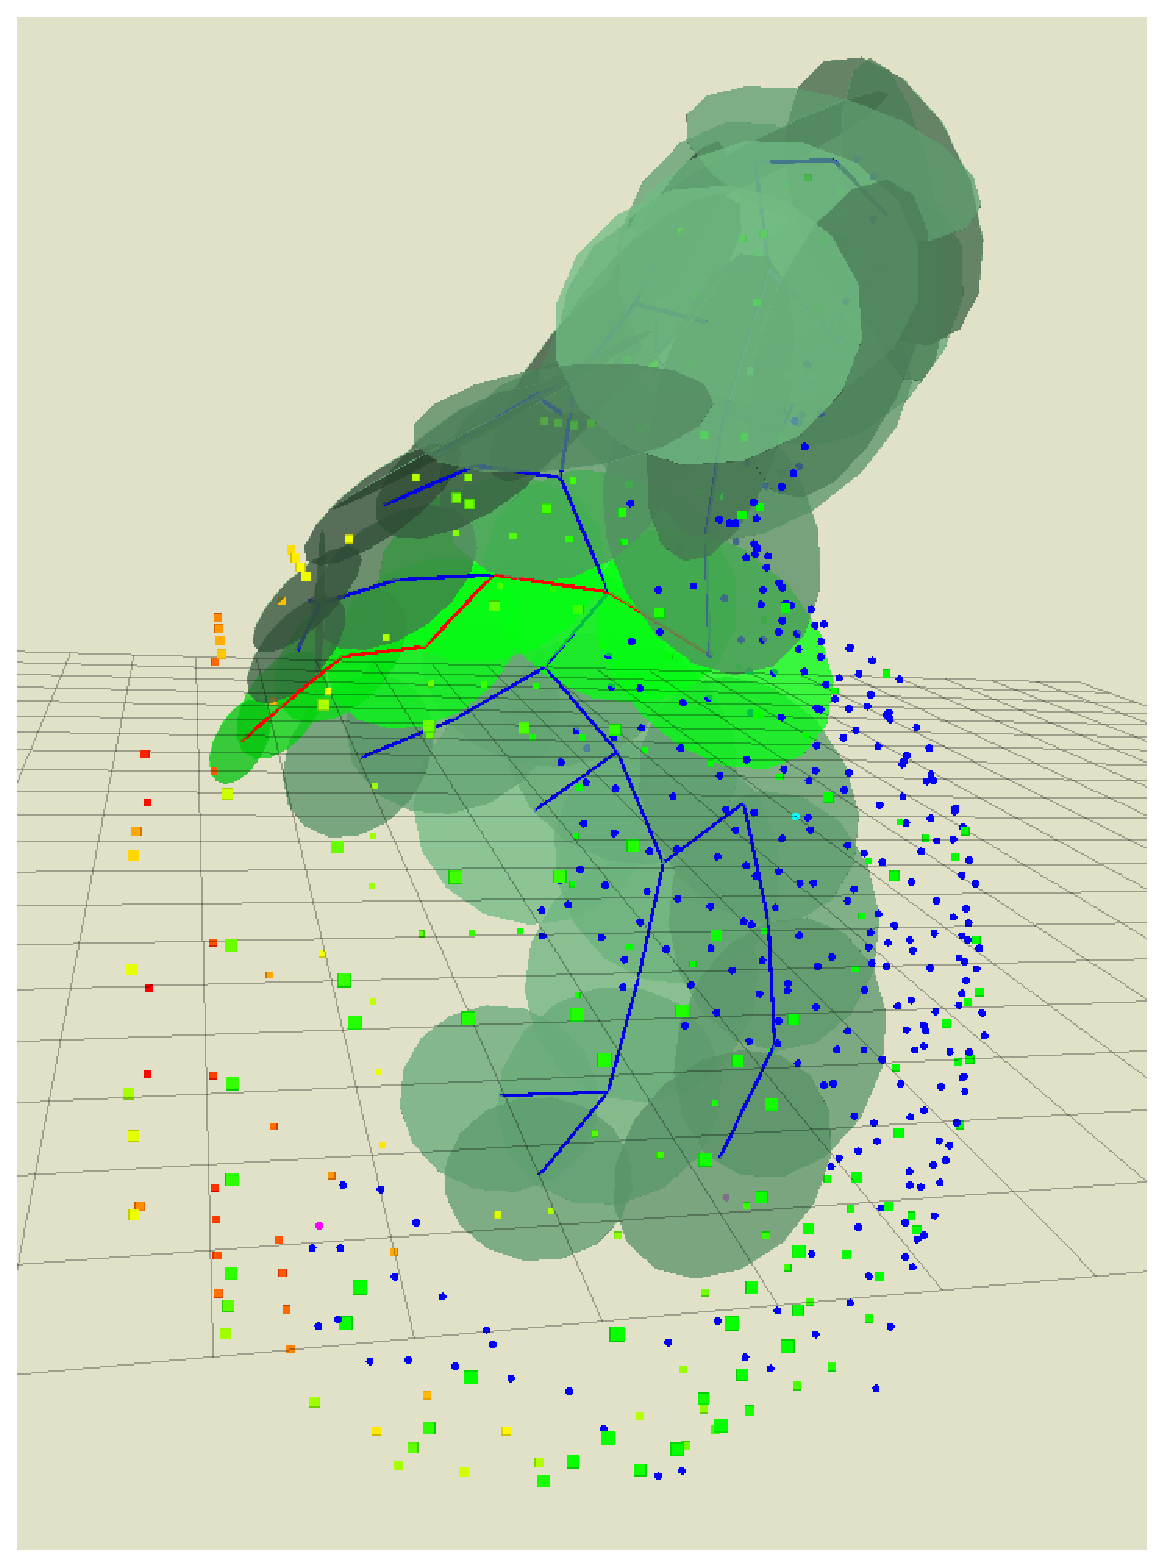
\includegraphics[width=0.45\linewidth]{funnelRRT2.eps}
    }
    \caption{RRT explorer on the funnel implicit surface. Solution is highlighted in green.}
    \label{fig:RRTfunnel}
    \todo[inline]{just added to see how it looks on the paper}
\end{figure}


























